\documentclass[12pt,a4paper]{article}
\topmargin -1.6cm
\addtolength{\textheight}{4cm}
\textwidth  15.5cm

\leftmargin      5mm
\rightmargin     5mm
\oddsidemargin   5mm
\evensidemargin  5mm

\usepackage{hyperref}
\usepackage{polski}
\usepackage[utf8]{inputenc}
\usepackage{graphicx}
\usepackage{units}
\usepackage{sty/style}
\usepackage{float}
\usepackage{mathtools}



\projekt{Modelowanie i identyfikacja}
\autor{Marcin Bober, 249426}
\przedmiot{Identyfikacja i modelowanie statystyczne}
\prowadzacy{Mgr inż. Maciej Filiński}

\begin{document}
\pdfpageheight   297mm
\pdfpagewidth    210mm

\StronaTytulowa
\SpisTresci

\pagebreak

\section{Generator liczb pseudolosowych}
  \subsection{Opis}
  Zadanie polega na implementacji generatora liczb pseudolosowych z rozkładu jednostajnego oraz analizie wyników uzyskanych z jego udziałem. Generator oparty jest na przekształceniu piłokształtnym o równaniu $X_{n+1} = X_n \cdot z - [X_n \cdot z]$ 

  \subsection{Wpływ wartości początkowej X na własności generatora}

  Wartość $Z$ ustawiona została na wartość 51. Wykorzystano 1000 próbek.

  \begin{figure}[H]
    \centering
    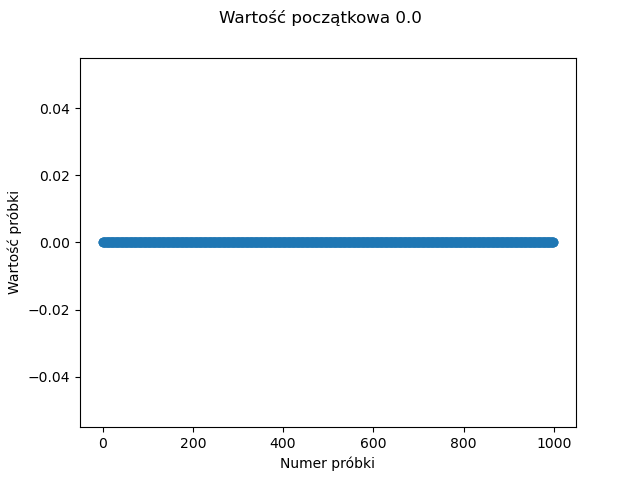
\includegraphics[height=0.3\textheight]{figures/Figure_1.png}
    \label{fig:1}
  \end{figure}

  \begin{figure}[H]
    \centering
    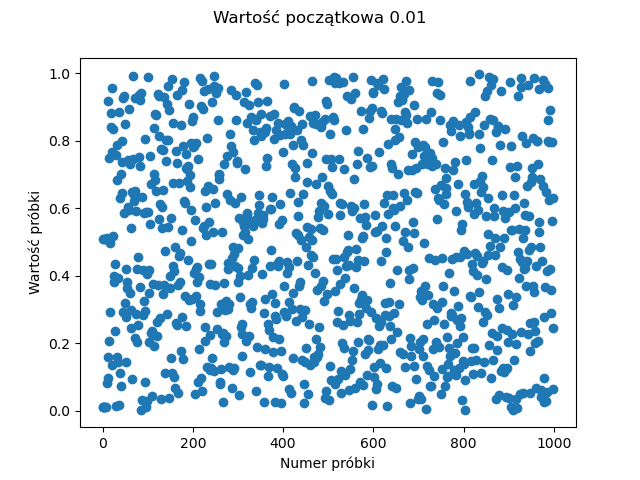
\includegraphics[height=0.3\textheight]{figures/Figure_2.png}
    \label{fig:2}
  \end{figure}

  \begin{figure}[H]
    \centering
    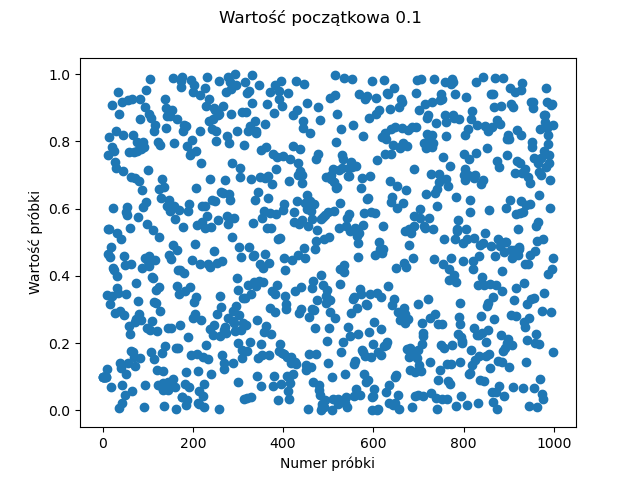
\includegraphics[height=0.3\textheight]{figures/Figure_3.png}
    \label{fig:3}
  \end{figure}

  \begin{figure}[H]
    \centering
    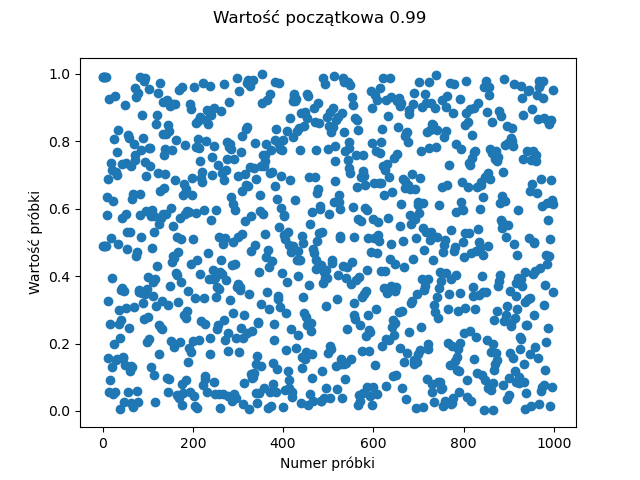
\includegraphics[height=0.3\textheight]{figures/Figure_4.png}
    \label{fig:4}
  \end{figure}

  \begin{figure}[H]
    \centering
    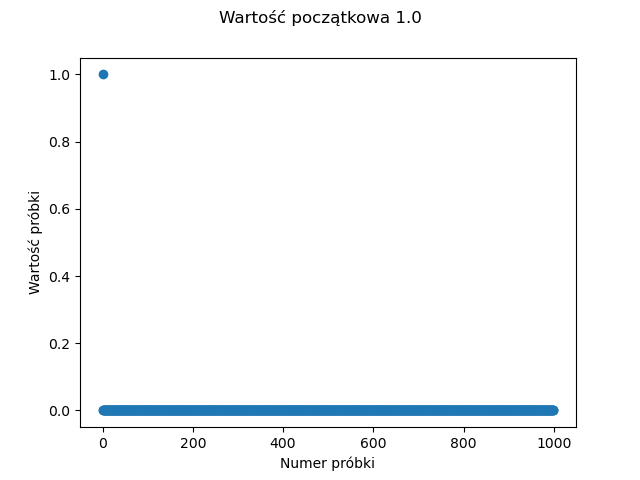
\includegraphics[height=0.3\textheight]{figures/Figure_5.png}
    \label{fig:5}
  \end{figure}
  
  \begin{itemize}
    \item Ustawienie wartości początkowej równej zero powoduje że wszystkie wygenerowane próbki są zerowe. (Patrz wykres \ref{fig:1}) Dzieje się tak ponieważ algorytm opiera się o obliczenie iloczynu liczb, których jednym ze składników jest zero.
    \item Wybór liczby całkowitej spowoduje że pierwsza próbka jest równa tej wartości, a wszystkie kolejne są zerowe (Patrz wykres \ref{fig:5}). Wynika to z faktu że obliczana jest reszta z dzielenia wartości przez jeden, która w taki wypadku zawsze równa jest zero.
    \item Zalecanym zakresem wyboru wartości początkowej jest przedział zawierający liczby większe od zera, z pominięciem liczb całkowitych.
  \end{itemize}

  \subsection{Wpływ parametru Z na własności generatora}

  Wartość $X_0$ ustawiona została na wartość 0,01. Wykorzystano 1000 próbek.

  \begin{figure}[H]
    \centering
    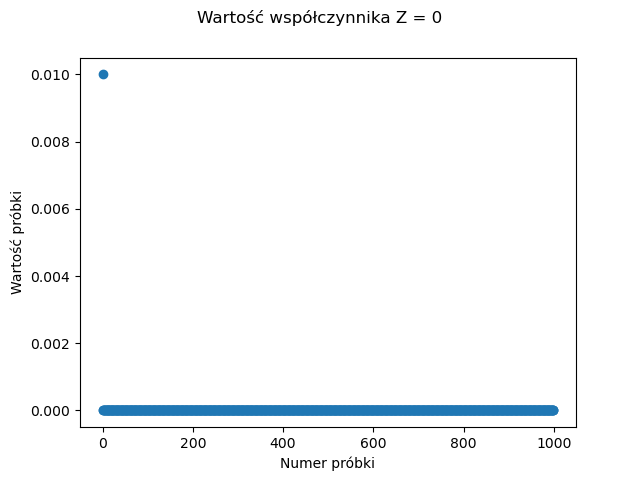
\includegraphics[height=0.3\textheight]{figures/Figure_6.png}
    \label{fig:6}
  \end{figure}

  \begin{figure}[H]
    \centering
    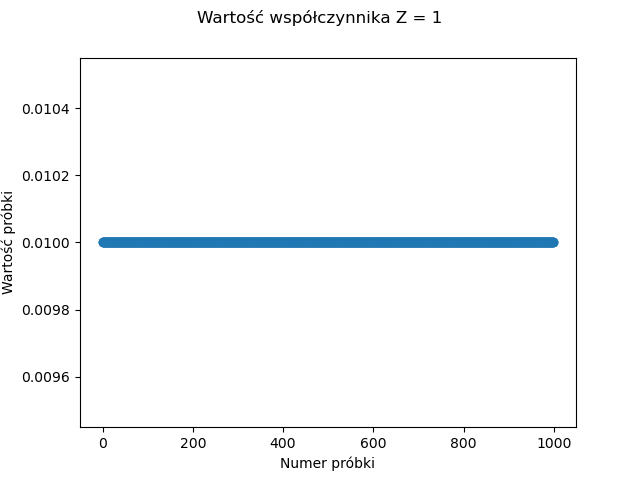
\includegraphics[height=0.3\textheight]{figures/Figure_7.png}
    \label{fig:7}
  \end{figure}

  \begin{figure}[H]
    \centering
    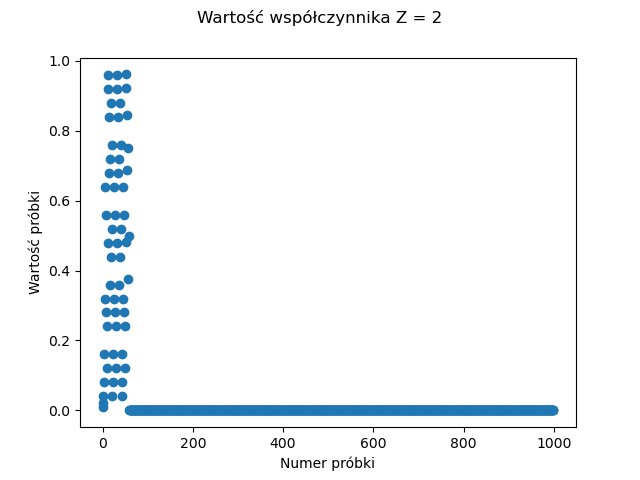
\includegraphics[height=0.3\textheight]{figures/Figure_8.png}
    \label{fig:8}
  \end{figure}

  \begin{figure}[H]
    \centering
    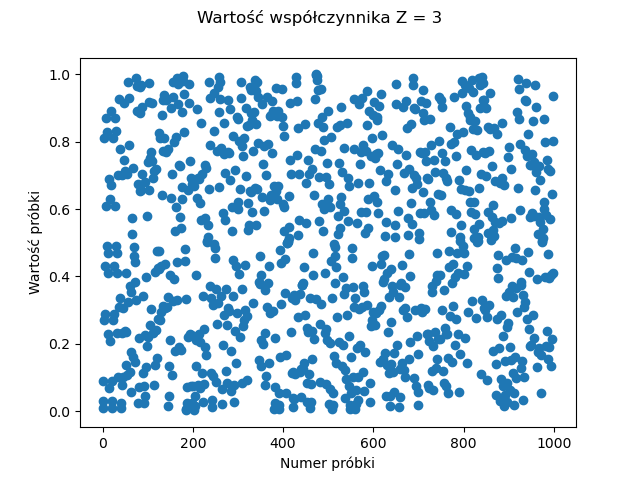
\includegraphics[height=0.3\textheight]{figures/Figure_9.png}
    \label{fig:9}
  \end{figure}
  
  \begin{itemize}
    \item Dla zerowego współczynnika $Z$ pierwsza próbka uzyskuje wartość początkowa, a kolejne są zerami. Wynika to z mnożenia tych wyników przez współczynnik $Z$ czyli zero.
    \item Gdy wartość $Z$ jest równa jedności, wszystkie otrzymane wyniki są identyczne z wartością startową.
    \item W przypadku wykorzystania liczb parzystych, uzyskiwane wyniki szybko trafiają na wartość zero, która powoduje zatrzymanie generowania kolejnych wartości losowych. 
    \item Najlepsze wyniki otrzymywane są dla współczynnika $Z$ będącego dużą liczbą pierwszą. 
  \end{itemize}

  \subsection{Okres generatora dla wybranych wartości Z}

  \begin{table}[h!]
    \centering
    \begin{tabular}{ c | c | c }
      $X_0$ & $Z$ & okres generatora  \\ 
      \hline
      0,1 & 1 & 1  \\  
      0,1 & 2 & 4  \\  
      0,1 & 3 & 4  \\  
      0,1 & 4 & 2  \\  
      0,1 & 5 & 1  \\
      0,1 & 6 & 1  \\
      0,1 & 7 & 4  \\
      0,1 & 8 & 4 
    \end{tabular}
    \caption{Okres generatora w zależności od wartości Z}
    \label{table:1}
  \end{table}

  \subsection{Podobieństwo histogramu ciągu wygenerowaych liczb, a gęstość rozkładu jednostajnego}


  \begin{figure}[H]
    \centering
    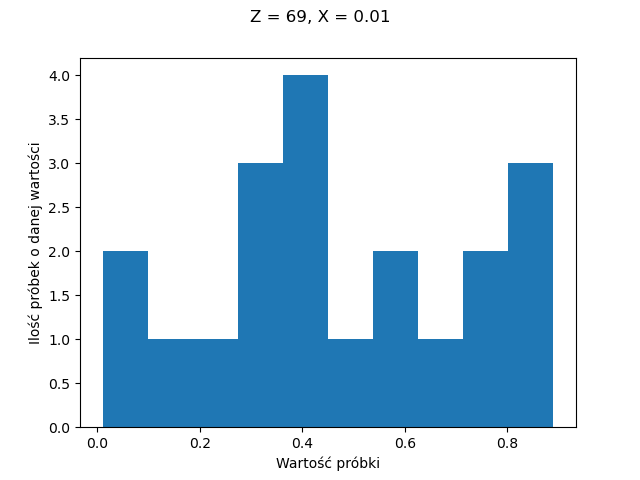
\includegraphics[height=0.25\textheight]{figures/Figure_10.png}
    \caption{Ilość wygenerowanych próbek - 20}
    \label{fig:10}
  \end{figure}

  \begin{figure}[H]
    \centering
    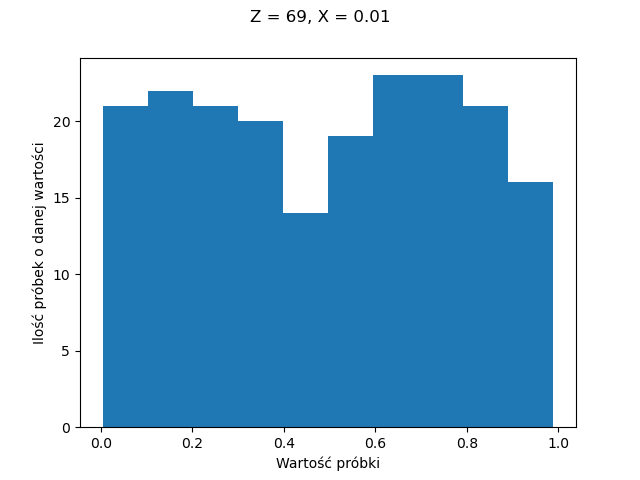
\includegraphics[height=0.25\textheight]{figures/Figure_11.png}
    \caption{Ilość wygenerowanych próbek - 200}
    \label{fig:11}
  \end{figure}

  \begin{figure}[H]
    \centering
    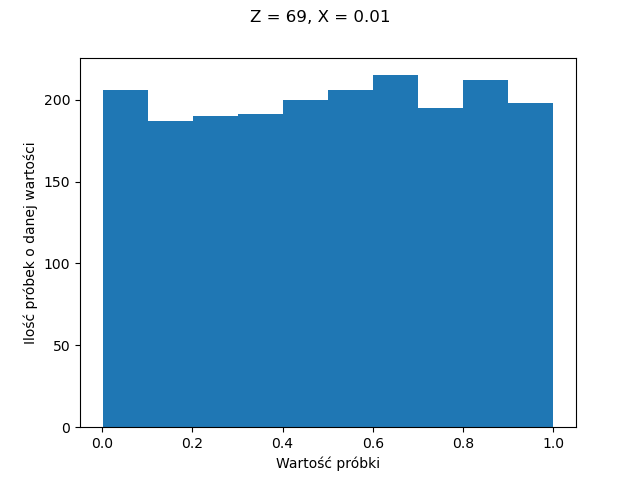
\includegraphics[height=0.25\textheight]{figures/Figure_12.png}
    \caption{Ilość wygenerowanych próbek - 2000}
    \label{fig:12}
  \end{figure}

  \begin{figure}[H]
    \centering
    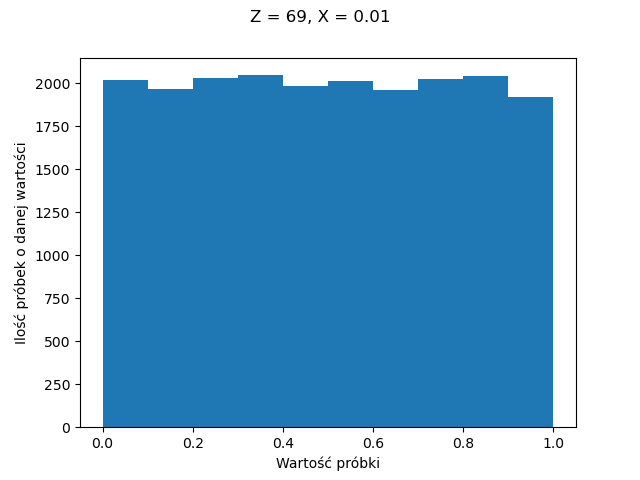
\includegraphics[height=0.25\textheight]{figures/Figure_13.png}
    \caption{Ilość wygenerowanych próbek - 20000}
    \label{fig:13}
  \end{figure}

  \begin{itemize}
    \item Im więcej wygenerowaych próbek tym mocniej histogram upodabnia się do gęstości prawdopodobieństwa rozkładu jednostajnego.  
  \end{itemize}

\section{Generator dany równaniem}

\subsection{Opis}
Zadanie polega na implementacji generatora liczb pseudolosowych oraz analizie wyników uzyskanych z jego udziałem. Generator oparty jest na równaniu: 

$X_{n+1}=(a_0X_{n} + a_1X_{n-1} + \ldots + a_{k}X_{n-k} + C)$mod $m$


\subsection{Zależność od współczynnika m}
Współczynnik $m$ odpowiada za zakres generowanych wartości.

\begin{figure}[H]
  \centering
  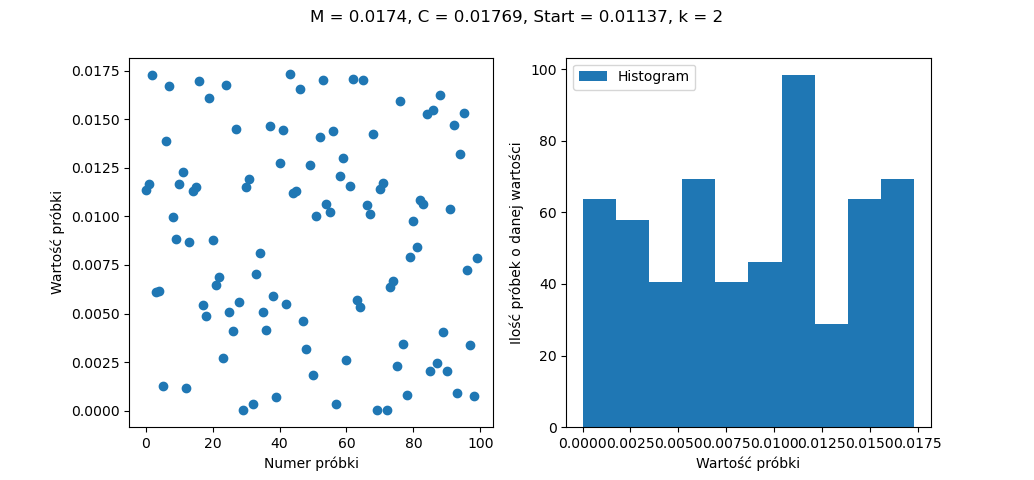
\includegraphics[width=1\textwidth]{figures/Figure_14.png}
  \caption{Zakres generowania liczb [0, 0.0174]}
  \label{fig:14}
\end{figure}

\begin{figure}[H]
  \centering
  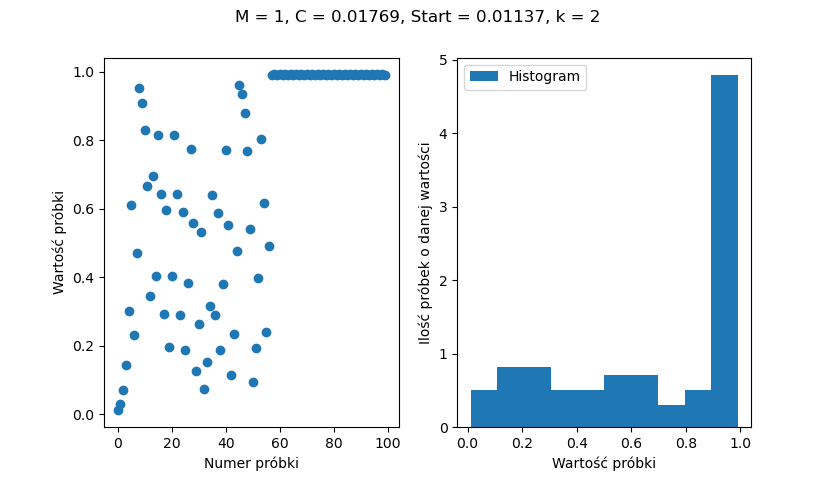
\includegraphics[width=1\textwidth]{figures/Figure_15.png}
  \caption{Zakres generowania liczb [0, 1]}
  \label{fig:15}
\end{figure}


\subsection{Zależność od współczynnika k}
Współczynnik $k$ odpowiada za ilość poprzednich próbek używanych podczas generowania nowych wartości. 

\begin{figure}[H]
  \centering
  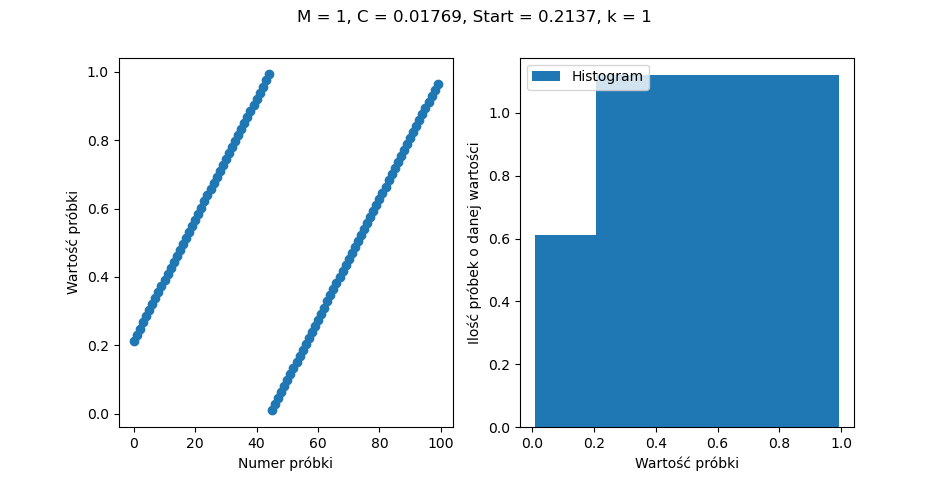
\includegraphics[width=0.8\textwidth]{figures/Figure_20.png}
  \caption{Współczynnik k=1}
  \label{fig:14}
\end{figure}

\begin{figure}[H]
  \centering
  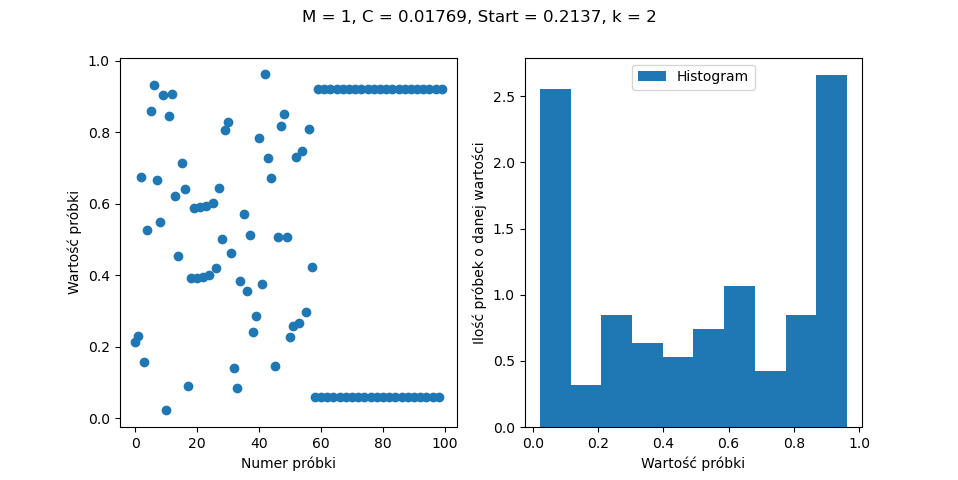
\includegraphics[width=0.8\textwidth]{figures/Figure_21.png}
  \caption{Współczynnik k=2}
  \label{fig:14}
\end{figure}

\begin{figure}[H]
  \centering
  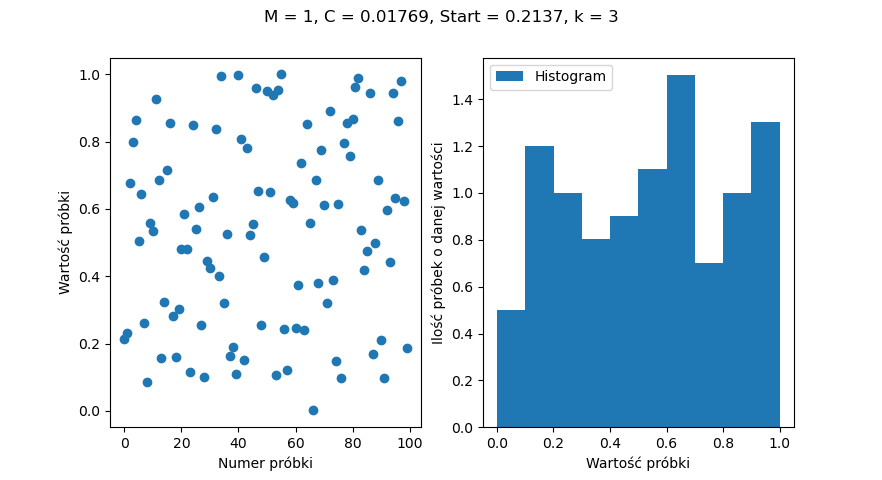
\includegraphics[width=0.8\textwidth]{figures/Figure_22.png}
  \caption{Współczynnik k=3}
  \label{fig:14}
\end{figure}


\begin{itemize}
  \item Współczynnik $m$ odpowiada za zakres generowanych wartości. Wybór liczby całkowitej może spowodować zatrzymanie generatora.
  \item Ustawienie współczynnika $k$ na wartość równą jeden uniemożliwia generowanie wartości losowych.
  \item Im większa wartość współczynnika $k$ tym lepsze wyniki generatora.
\end{itemize}

\section{Metoda odwracania dystrybuanty}
  \subsection{Opis}
    Metoda odwracania dystrybuanty polega na odwróceniu funkcji dystrybuanty. Do uzyskania funkcji dystrybuanty posłużymy się całkowaniem funkcji opisującej gęstość prawdopodobieństwa analizowanego rozkładu.

  \subsection{Rozkład numer 1}
  
    Równanie funkcji rozkładu gęstość prawdopodobieństwa:
    \begin{equation}
      f(x) = \begin{cases}
          2x \quad dla \quad x  \in [0,1]\\
          0 \quad dla \quad x  \in (-\infty, 0) \cup (1, \infty)\\
        \end{cases}   
    \end{equation}

    Dystrybuanta:
    \begin{equation}
      F(x) = \begin{cases}
          0 \quad dla \quad x  \in (-\infty, 0)\\
          x^2 \quad dla \quad x  \in [0, 1]\\
          1 \quad dla \quad x  \in (1, \infty)\\
        \end{cases}   
    \end{equation}

    Odwrotna dystrybuanta:
    \begin{equation}
      F^{-1}(y) = \sqrt{y}.
    \end{equation}

  \begin{figure}[H]
    \centering
    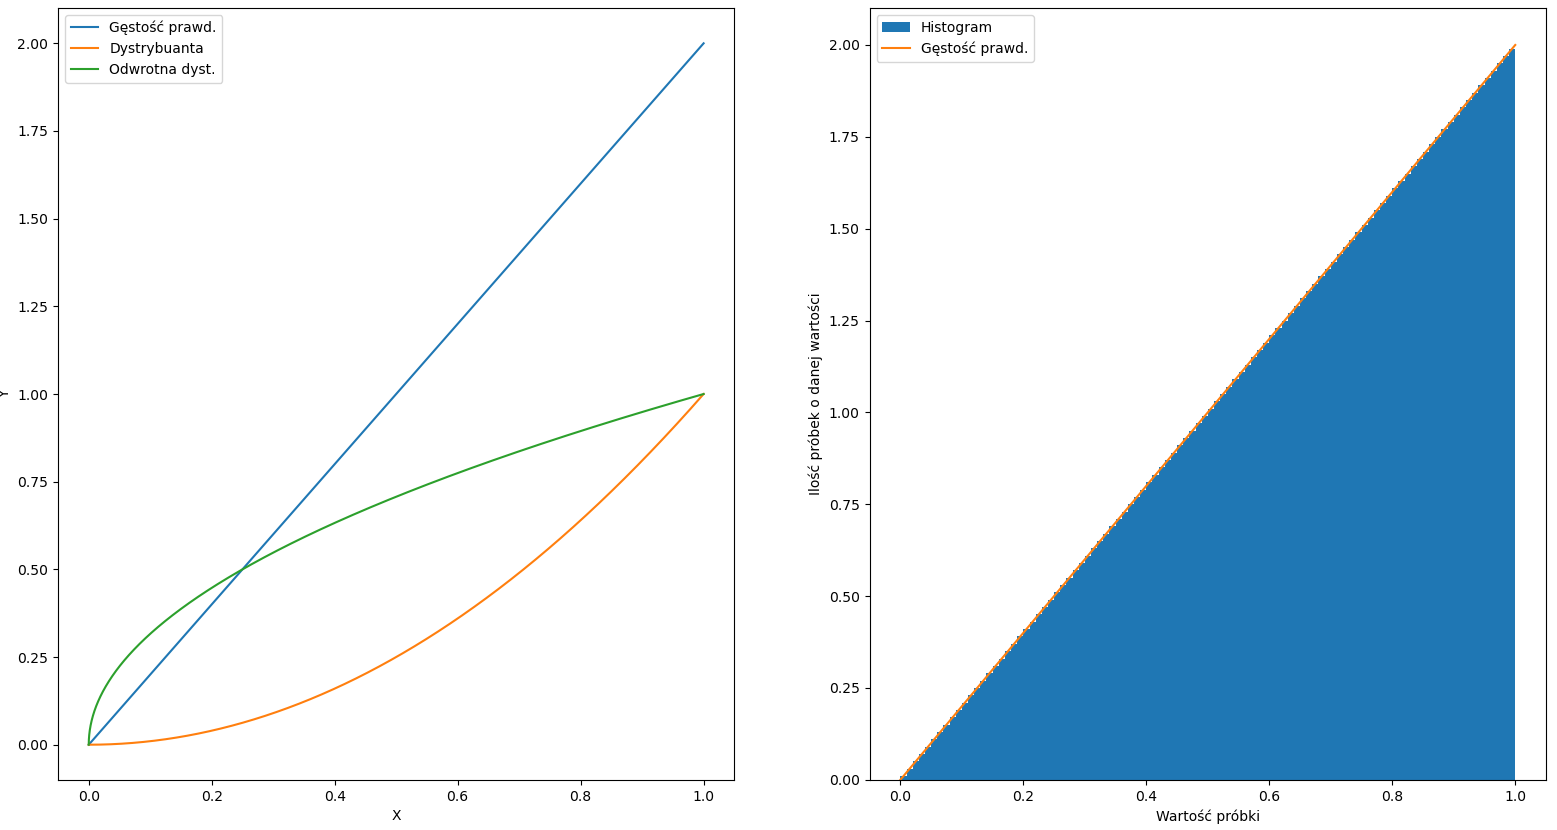
\includegraphics[width=1\textwidth]{figures/Figure_16.png}
    \label{fig:16}
  \end{figure}


  \subsection{Rozkład numer 2}
  
  Równanie funkcji rozkładu gęstość prawdopodobieństwa:
  \begin{equation}
    f(x) = \begin{cases}
        x + 1 \quad dla \quad x  \in (-1, 0)\\
        -x + 1 \quad dla \quad x  \in [0, 1)\\
        0 \quad dla \quad x  \notin (-1, 1)\\
      \end{cases}   
  \end{equation}

  Dystrybuanta:
  \begin{equation}
    F(x) = \begin{cases}
        \frac{1}{2} - \frac{x^2}{2} + x \quad dla \quad x  \in [0, 1)\\
        \frac{1}{2} + \frac{x^2}{2} + x \quad dla \quad x  \in (-1, 0)\\
        0 \quad dla \quad x  \in (-\infty, -1]\\
        1 \quad dla \quad x  \in [1, \infty)\\
      \end{cases}   
  \end{equation}

  Odwrotna dystrybuanta:
  \begin{equation}
    F^{-1}(y) = \begin{cases}
          \sqrt{2y} -1 \quad dla \quad x  \in [0, \frac{1}{2}]\\
          1 -\sqrt{2 - 2y} \quad dla \quad x  \in (\frac{1}{2}, 1]\\
        \end{cases}   
  \end{equation}

  \begin{figure}[H]
    \centering
    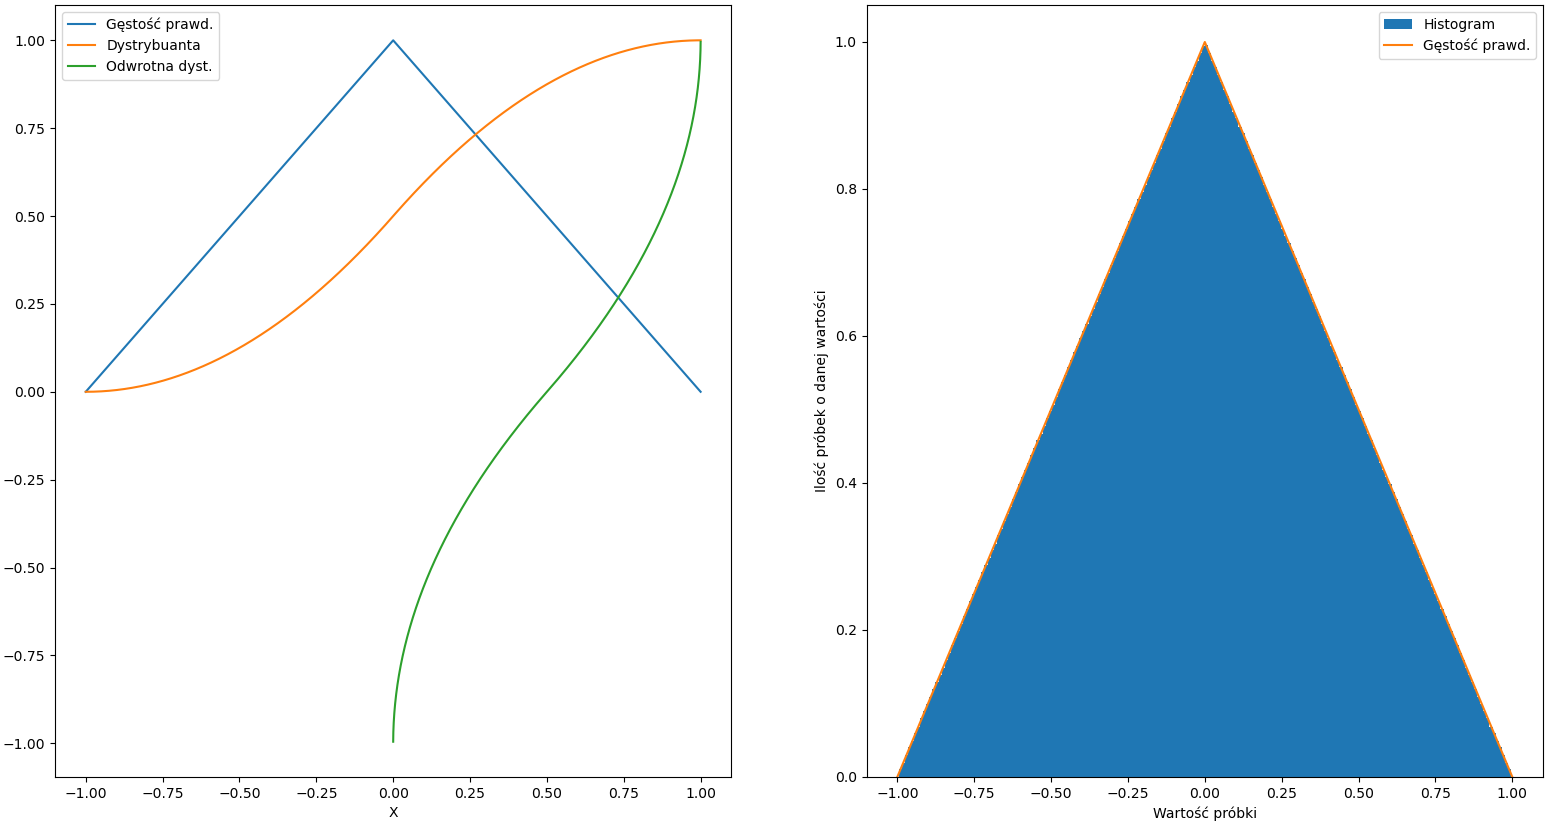
\includegraphics[width=1\textwidth]{figures/Figure_17.png}
    \label{fig:17}
  \end{figure}

  \subsection{Rozkład wykładniczy}
  
  Równanie funkcji rozkładu gęstość prawdopodobieństwa:
  \begin{equation}
    f(x) = e^{-x}  \quad dla \quad x  \in [0, \infty)
  \end{equation}

  Dystrybuanta:
  \begin{equation}
    F(x) = 1 - e^{-x}  \quad dla \quad x  \in [0, \infty)
  \end{equation}

  Odwrotna dystrybuanta:
  \begin{equation}
    F^{-1}(y) = -ln(1 - y)  \quad dla \quad x  \in [0, \infty)
  \end{equation}


  \begin{figure}[H]
    \centering
    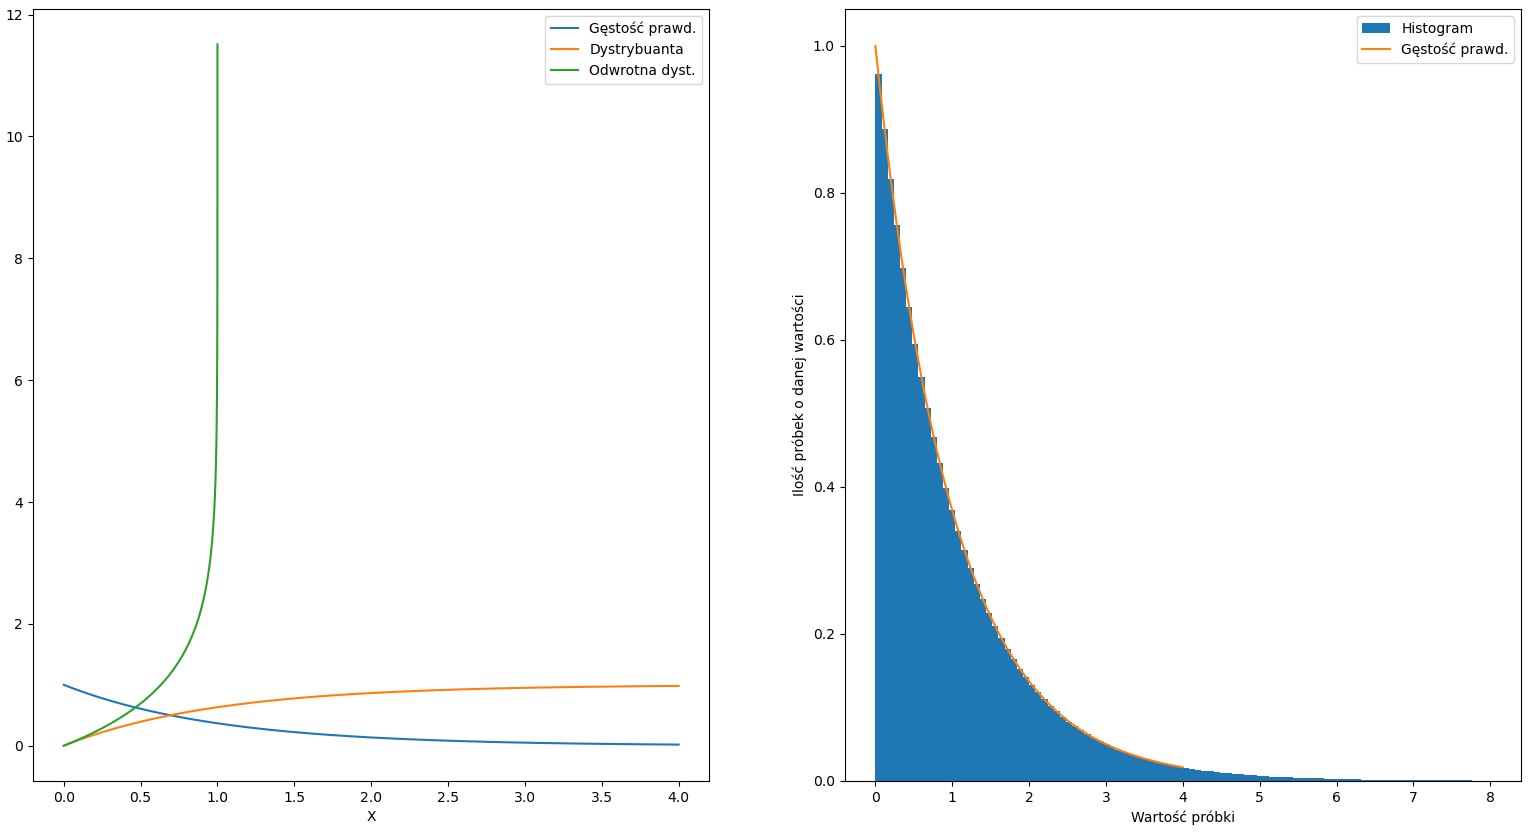
\includegraphics[width=1\textwidth]{figures/Figure_18.png}
    \label{fig:18}
  \end{figure}

  \subsection{Rozkład Laplace'a}
  
  Równanie funkcji rozkładu gęstość prawdopodobieństwa:
  \begin{equation}
    F(x) = \frac{1}{2} e^{-|x|} 
  \end{equation}

  Dystrybuanta:
  \begin{equation}
      F^{-1}(y) = \begin{cases}
            \frac{1}{2} + \frac{1}{2} (1 - e^{-x})  \quad dla \quad x  \in [0, \infty)\\
            \frac{1}{2} - \frac{1}{2} (1 - e^{-x})  \quad dla \quad x  \in (-\infty, 0)\\
          \end{cases}   
  \end{equation}

  Odwrotna dystrybuanta:
    \begin{equation}
      F^{-1}(y) = \begin{cases}
            -ln(1 - y) \quad dla \quad x  \in [0, \infty)\\
            ln(1 + y) \quad dla \quad x  \in (-\infty, 0)\\
          \end{cases}   
    \end{equation}

  \begin{figure}[H]
    \centering
    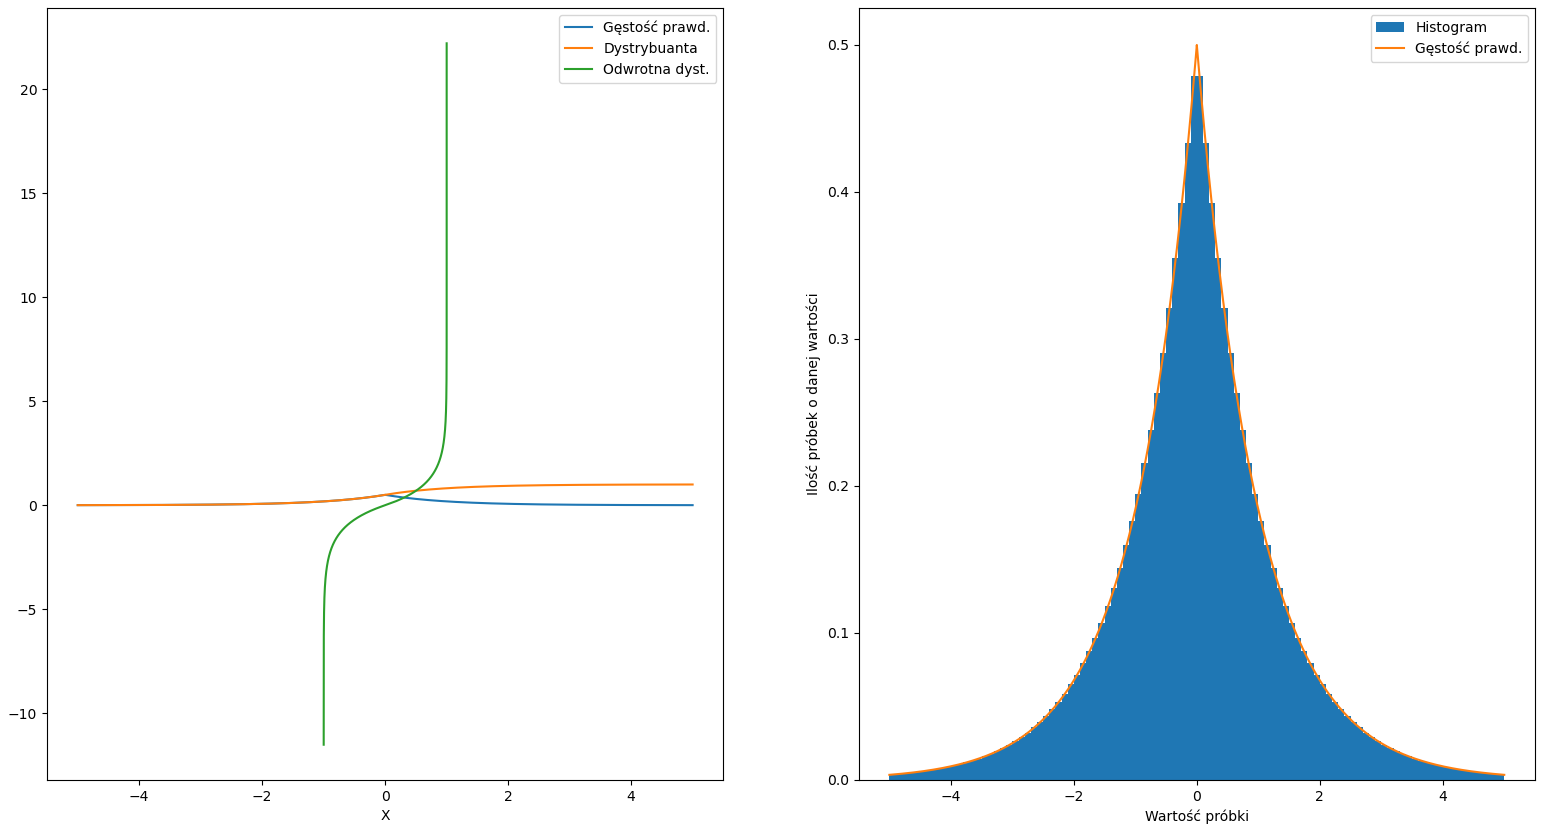
\includegraphics[width=1\textwidth]{figures/Figure_19.png}
    \label{fig:19}
  \end{figure}


\section{Metoda odrzucania}
  \subsection{Rozkład numer 1}
    
  Równanie funkcji rozkładu gęstość prawdopodobieństwa:
  \begin{equation}
    f(x) = \begin{cases}
        x + 1 \quad dla \quad x  \in (-1, 0]\\
        -x + 1 \quad dla \quad x  \in (0, 1]\\
        0 \quad dla \quad x  \in (-\infty, -1] \cup (1, \infty)\\
      \end{cases}   
  \end{equation}

  Przybliżenie funkcji f(x) z użyciem funkcji g(x):
  \begin{equation}
    g(x) = \frac{1}{2} e^{-|x|}
  \end{equation}

  Odwrotna dystrybuanta:
  \begin{equation}
    G^{-1}(y) =   \quad dla \quad x  \in [0, \infty)
    \begin{cases}
      ln(2x) \quad dla \quad x  \in (-\infty, \frac{1}{2}]\\
      -ln(2-2x) \quad dla \quad x  \in (\frac{1}{2}, \infty)\\
    \end{cases} 
  \end{equation}

  \begin{figure}[H]
    \centering
    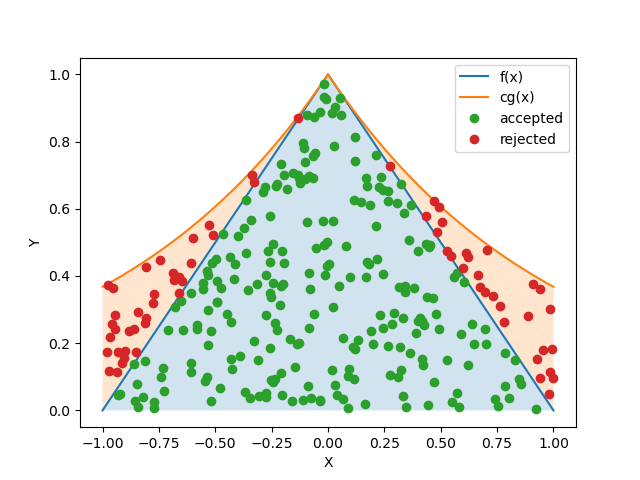
\includegraphics[height=0.4\textheight]{figures/Figure_23.png}
    \label{fig:23}
    \caption{Generacja próbek rozkładu 1}
  \end{figure}

  \begin{figure}[H]
    \centering
    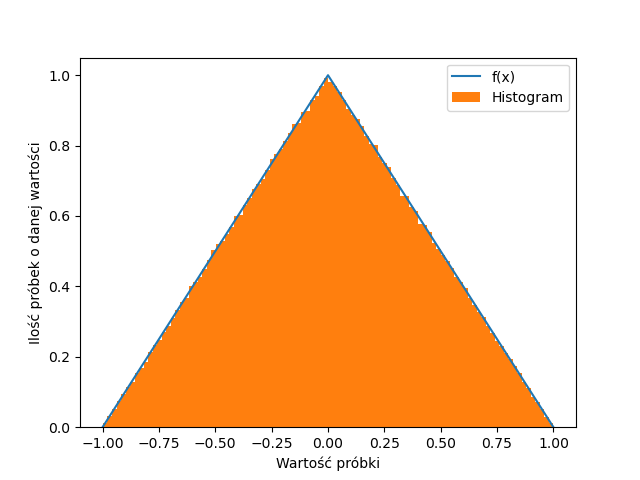
\includegraphics[height=0.4\textheight]{figures/Figure_24.png}
    \label{fig:24}
    \caption{Histogram rozkładu 1}

  \end{figure}

  \subsection{Rozkład numer 2}
      
  Równanie funkcji rozkładu gęstość prawdopodobieństwa:
  \begin{equation}
    f(x) = \begin{cases}
        50 \quad dla \quad x  \in (0, \frac{1}{100}]\\
        c \quad dla \quad x  \in (\frac{1}{100}, 1]\\
      \end{cases}   
  \end{equation}

  Współczynnik $c$ został wyznaczony w następujący sposób:
  \begin{equation}
    50 \cdot \frac{1}{100} + c \cdot 1 - \frac{1}{100} = 1
  \end{equation}

  \begin{equation}
    c \cdot 1 - \frac{1}{100} = 1 - \frac{50}{100}
  \end{equation}

  \begin{equation}
    c = \frac{0.5}{\frac{99}{100}}
  \end{equation}
  

  Przybliżenie funkcji f(x) z użyciem funkcji g(x):
  \begin{equation}
    g(x) = 50 \cdot e^{-4.1 \cdot (x-0.01)}  \quad dla \quad x  \in [0, \infty) \\
  \end{equation}

  Odwrotna dystrybuanta:
  \begin{equation}
    g(x) = -0.244 \cdot ln(0.01919 \cdot x)
  \end{equation}

  \begin{figure}[H]
    \centering
    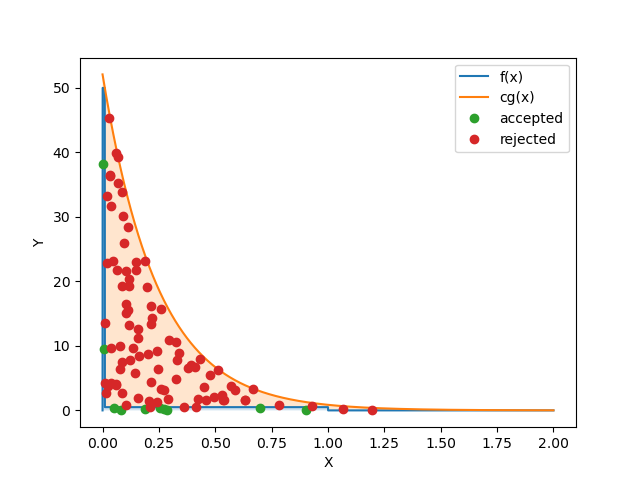
\includegraphics[height=0.4\textheight]{figures/Figure_25.png}
    \label{fig:25}
    \caption{Generacja próbek rozkładu 2}
  \end{figure}

  \begin{figure}[H]
    \centering
    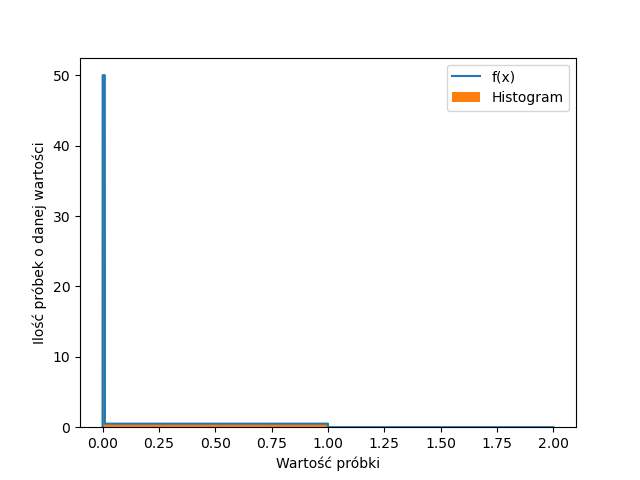
\includegraphics[height=0.4\textheight]{figures/Figure_26.png}
    \label{fig:26}
    \caption{Histogram rozkładu 2}

  \end{figure}


\subsection{Półokrąg}
      
Równanie funkcji rozkładu gęstość prawdopodobieństwa:
\begin{equation}
  f(x) = \sqrt{r^2 - x^2 }
\end{equation}

Przybliżenie funkcji f(x) z użyciem funkcji g(x):
\begin{equation}
  g(x) = 1  \quad dla \quad x  \in [-1, 1] \\
\end{equation}

\begin{figure}[H]
  \centering
  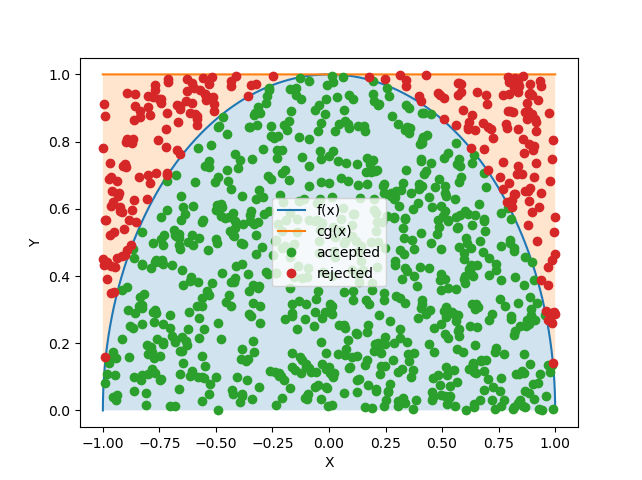
\includegraphics[height=0.4\textheight]{figures/Figure_27.png}
  \label{fig:27}
  \caption{Generacja próbek dla półokręgu}
\end{figure}

\begin{figure}[H]
  \centering
  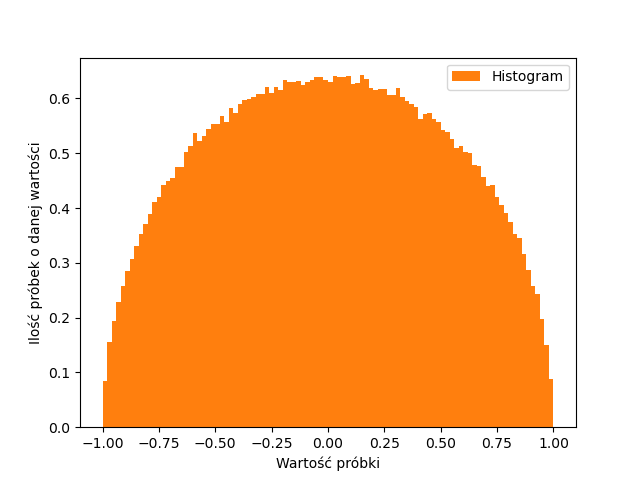
\includegraphics[height=0.4\textheight]{figures/Figure_28.png}
  \label{fig:28}
  \caption{Histogram rozkładu dla półokręgu}

\end{figure}

\subsection{Rozkład Normalny}
      
Równanie funkcji rozkładu gęstość prawdopodobieństwa:
\begin{equation}
  f(x) = \frac{1}{\sqrt{2 \pi}} \cdot e^{\frac{-x^2}{2}}
\end{equation}


Przybliżenie funkcji f(x) z użyciem funkcji g(x):
\begin{equation}
  g(x) = \sqrt{\frac{2e}{\pi}} \cdot \frac{1}{2} \cdot e^{-|x|}
\end{equation}

Odwrotna dystrybuanta:
\begin{equation}
  g(x) = \begin{cases}
      ln(2x) \quad dla \quad x  \in (-\infty, \frac{1}{2}]\\
      -ln(2+2x) \quad dla \quad x  \in (\frac{1}{2}, \infty)\\
    \end{cases}   
\end{equation}

\begin{figure}[H]
  \centering
  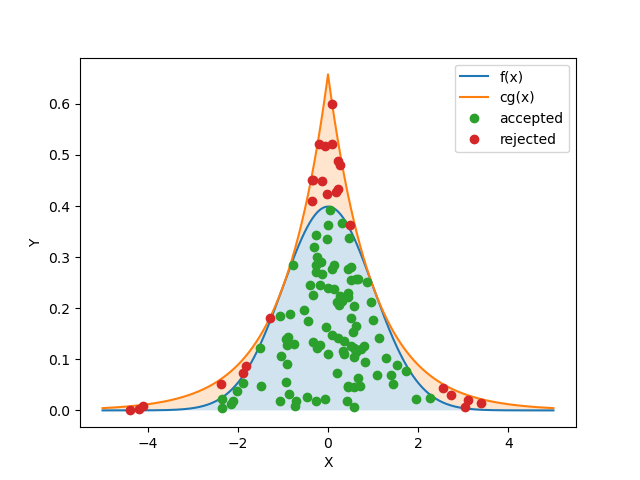
\includegraphics[height=0.4\textheight]{figures/Figure_29.png}
  \label{fig:29}
  \caption{Generacja próbek rozkładu normalnego}
\end{figure}

\begin{figure}[H]
  \centering
  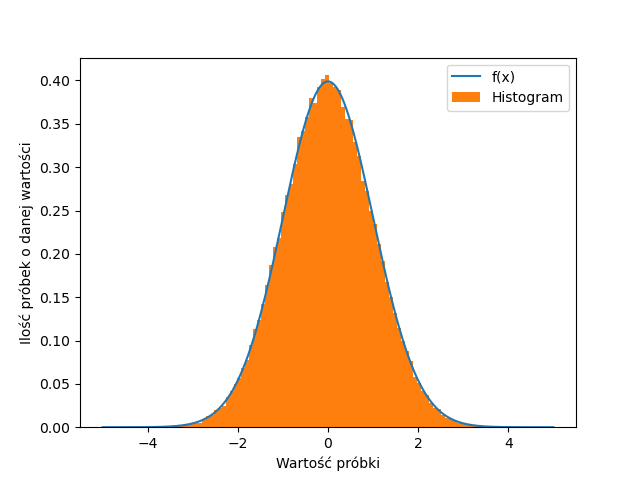
\includegraphics[height=0.4\textheight]{figures/Figure_30.png}
  \label{fig:30}
  \caption{Histogram rozkładu normalnego}

\end{figure}

\subsection{Wnioski}
\begin{itemize}
  \item Metoda eliminacji jest metodą stratna ponieważ w zależności od dobranej funkcji g(x), odrzucana jest pewna ilość losowań.
  \item Im lepiej dobierzemy funkcję pomocniczą tym większa efektywność generatora.
  \item Funkcja pomocnicza musi być odwrócona, więc należy dobierać funkcje możliwie trywialne.
  \item Stała $C$ może być dobrana dowolnie duża, ale wyznaczenie jej analitycznie minimalizuje straty.
\end{itemize}

\section{Estymacja}
\section{Podsumowanie}

\end{document}